\documentclass{beamer}
\usepackage[utf8]{inputenc}
\usepackage{colortbl}
\usepackage{multimedia}
\usetheme{JuanLesPins}
\mode<presentation>
\useoutertheme{smoothtree}
\usecolortheme{whale}
\usecolortheme{orchid}
\useinnertheme[shadow=true]{rounded}
% profondeur table des matieres
\setcounter{tocdepth}{1}
\setbeamerfont{block title}{size={}}
\title{Projet Tuteuré \\Gestion centralisée de machines virtuelles}
\author{Augustin Bocca Julien Tournois\\Sébastien Michaux Mathieu Lamouroux}
\institute{IUT de Nancy Charlemagne}
%\addtobeamertemplate{footline}{\insertframenumber/\inserttotalframenumber}
\begin{document}

\AtBeginSection[]
{
  \begin{frame}<beamer>
    \frametitle{Plan}
    \tableofcontents[currentsection,currentsubsection,hideothersubsections]
  \end{frame}
}

\begin{frame}
  \titlepage
\end{frame}

\begin{frame}
    \frametitle{Plan}
    \tableofcontents
\end{frame}

%%%%%%%%%%%%%%%%%%%%%%%%%%%%%%%%%%%%%%%%%%%%%%%%%%%%%%%%%%%%
\section{Le contexte}
\subsection{Le projet}
\begin{frame}{Le projet tuteuré}
 %%%% trouver une boite
\begin{block}{Intitulé}
Mettre en place, évaluer et comparer différents outils de gestion centralisée de machines virtuelles.
\end{block}
\pause
\begin{block}{Résultats attendus}
  \begin{itemize}
    \item guide d'installation et d'utilisation synthétique
\pause
    \item scripts
\pause
    \item démos à grande échelle sur grid5000
\pause
    \item avis critique
   \end{itemize}
\end{block}
\end{frame}

\subsection{Grid5000}
\begin{frame}{La plateforme Grid5000}
%%%%%%%%% PHOTO
\begin{block}{Vue d'ensemble}
  \begin{itemize}
    \item Grille Informatique
\pause
    \item Dix sites en France
\pause
    \item Réliés par RENATER
\pause
    \item Objectif scientifique
  \end{itemize}
\end{block}
\end{frame}

\begin{frame}{Architecture type d'un site}
  \begin{center}
    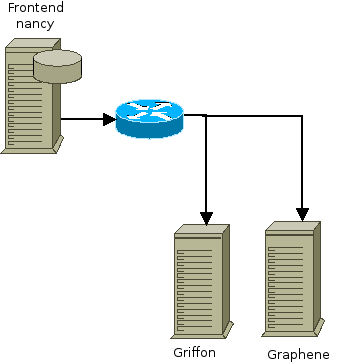
\includegraphics[width=180pt]{images_presentation/archi.png}
  \end{center}
\end{frame}

\begin{frame}{Connexion à un site}
  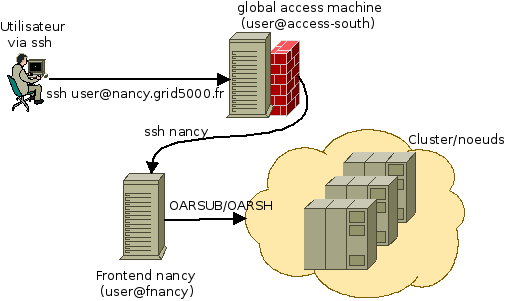
\includegraphics[width=330pt]{images_presentation/plan_site.png}
\end{frame}


%%%%%%%%%%%%%%%%%%%%%%%%%%%%%%%%%%%%%%%%%%%%%%%%%%%%%%%%%%%%
\section{La virtualisation}
\subsection{Historique}
\begin{frame}{Il était une fois la virtualisation...}
  \begin{description}
    \item[1960 : ] inventée par IBM pour optimiser l'utilisation du matériel sur les serveurs
\pause
    \item[1990 : ] VMware porte le concept sur les plateformes x86
\pause
    \item[Aujourd'hui : ] VMware se positionne en tant que leader du marché.
  \end{description}
\end{frame}

\subsection{Enjeux}
\begin{frame}{Pourquoi virtualisé?}
  Et c'est facile.
\end{frame}

%%%%%%%%%%%%%%%%%%%%%%%%%%%%%%%%%%%%%%%%%%%%%%%%%%%%%%%%%%%%
\section{Logiciels testés}
\subsection{Ganeti}
%%%%%%%% LOGO
\chapter{Ganeti}
\section{Introduction}
Ganeti est un outil de gestion de machines virtuelles se basant sur les technologies de virtualisation existantes comme XEN et KVM.\\
<<<<<<< HEAD
Ganeti n�cessite un logiciel de virtualisation pr�-install� sur les serveurs afin de pouvoir fonctionner. Une fois install�, 
l'outil prendra en charge la partie gestion des instances virtuelles (Xen DomU), par exemple, la gestion de cr�ation de disque, 
l'installation du syst�me d'exploitation (en coop�ration avec les scripts d'installation du syst�me d'exploitation 
sp�cifique), et le d�marrage, l'arr�t, le basculement entre les syst�mes physiques. Il a �t� con�u pour faciliter la gestion de 
cluster de serveurs virtuels et de fournir une r�cup�ration rapide et simple.


\section {Installation}
\subsection {Modification des sources}
Nous avons intall� ganeti � partir de la branche testing de debian. Pour des raisons techniques le syst�me est squeeze. Pour cela il faut ajouter les sources de testing dans le fichier /etc/apt/sources.list :
=======
%Ganeti nécessite un logiciel de virtualisation pré-installé sur les serveurs afin de pouvoir fonctionner. Une fois installé, l'outil prendra en charge la partie gestion des instances virtuelles (Xen DomU), par exemple, la gestion de création de disque, l'installation du système d'exploitation (en coopération avec les scripts d'installation du système d'exploitation spécifique), et le démarrage, l'arrêt, le basculement entre les systèmes physiques. Il a été conçu pour faciliter la gestion de cluster de serveurs virtuels et de fournir une récupération rapide et simple.

\section{Installation}
\subsection{Modification des sources}
Nous avons intallé ganeti à partir de la branche testing de debian. Pour des raisons techniques le système est squeeze. Pour cela il faut ajouter les sources de testing dans le fichier /etc/apt/sources.list :
>>>>>>> bdb35216a929de37c6411ee8791b131964b0fad8
\begin{lstlisting}
##Wheezy
deb http://ftp.fr.debian.org/debian/ wheezy main contrib non-free
deb-src http://ftp.fr.debian.org/debian/ wheezy main contrib non-free

## wheezy security
deb http://security.debian.org/ wheezy/updates main contrib non-free
deb-src http://security.debian.org/ wheezy/updates main contrib non-free
\end{lstlisting}

IL faut ensuite cr�er le fichier de pr�f�rence de apt dans le r�pertoire /etc/apt/apt.conf.d. Nous avons appel� le  fichier 80default-distrib (le nom du fichier est libre). Il faut ajouter cette ligne au fichier qui d�fini la branche stable comme la branche par d�faut :
\begin{lstlisting}
APT::Default-Release "stable";
\end{lstlisting}

<<<<<<< HEAD
\subsection {Mise � jour et installation}
On peut enfin alors mettre le syst�me � jour et installer ganeti :
=======
\subsection{Mise à jour et installation}
On peut enfin alors mettre le système à jour et installer ganeti :
>>>>>>> bdb35216a929de37c6411ee8791b131964b0fad8

\begin{lstlisting}
apt-get update && apt-get dist-upgrade -q -y --force-yes
apt-get -t testing install -q -y --force-yes ganeti2 ganeti-htools ganeti-instance-debootstrap
\end{lstlisting}

\section{Configuration}

La configuration est l'�tape la plus complexe.

\subsection{Configuration du fichier hosts}

Dans le fichier hosts il faut renseigner l'adresse et le nom complet du node primaire de cette mani�re :
\begin{lstlisting}
172.16.68.10    griffon-10.nancy.grid5000.fr griffon-10
\end{lstlisting}
\subsection{Copie de vmlinuz-2.6.32-5-xen-amd64 et initrd.img-2.6.32-5-xen-amd64}
Dans /etc/boot copier les fichiers vmlinuz-2.6.32-5-xen-amd64 et initrd.img-2.6.32-5-xen-amd64 :
\begin{lstlisting}
cp vmlinuz-2.6.32-5-xen-amd64 vmlinuz-2.6-xenU
cp initrd.img-2.6.32-5-xen-amd64 initrd.img-2.6-xenU
\end{lstlisting}

<<<<<<< HEAD
\subsection {Cr�ation du bridge xen-br0}

\subsection {Cr�ation du LVM}
=======
\subsection{Création du bridge xen-br0}
BLABLABLA
\subsection{Création du LVM}
>>>>>>> bdb35216a929de37c6411ee8791b131964b0fad8

Ganeti requi�re un LVM d'au moins 20Go pour fonctionner.

Sur les neud de grid5000 il est possible de cr�er un tel LVM sur la partition /dev/sd5.
\begin{lstlisting}
umount /dev/sda5
pvcreate /dev/sda5
vgcreate xenvg /dev/sda5
\end{lstlisting}
On a cr�� un VG qui se nome xenvg sur /dev/sda5.

\subsection{Edition de /usr/share/ganeti/os/debootstrap/common.sh}

Il est n�cessaire d'�diter ce fichier pour que ganeti puisse cr�er des instances :

<<<<<<< HEAD
Par defaut le mirroir utilis� par ganeti est http://ftp.us.debian.org/debian/. Sur Grid5000 les depots US sont bloqu�s. Il faut donc indiquer les depots francais.
On indique aussi l'adresse du  proxy de grid5000.
On peut choisir la version de Debian que l'on souhaite installer. Ici nous avons opter pour squeeze.
L'architecture que nous choisi est amd64, car l'hote la supporte.
La variable : extra_pkdg permet d'installer des paquets suppl�mentaires.
=======
%Par défaut le mirroir utilisé par ganeti est http://ftp.us.debian.org/debian/. Sur Grid5000 les depots US sont bloqués. Il faut donc indiquer les depots francais. On indique aussi l'adresse du  proxy de grid5000. On peut choisir la version de Debian que l'on souhaite installer. Ici nous avons opter pour squeeze. L'architecture que nous choisi est amd64, car l'hôte la supporte. La variable : EXTRA_PKGS permet d'installer des paquets supplémentaires.
>>>>>>> bdb35216a929de37c6411ee8791b131964b0fad8

\subsection{Configuration et initialisation du cluster}
L'initialisation du cluster se fait avec la commande gnt-cluster init clusterX
\begin{lstlisting}
#initialisation du cluster
gnt-cluster init --no-drbd-storage --nic-parameters link=eth0 cluster1
\end{lstlisting}
Ici nous avons pr�cis� les options --no-drbd-storage --nic-parameters link=eth0.
La premi�re permet d'utiliser ganeti sans utiliser la haute disponibilit�.
La seconde permet de pr�ciser un autre bridge que xen-br0

Enfin il faut renseigner le inird et le root_path, cela est n�cessaire pour la cr�ation des instances :
\begin{lstlisting}
gnt-cluster modify --hypervisor-parameter xen-pvm:initrd_path='/boot/initrd.img-2.6-xenU'
gnt-cluster modify --hypervisor-parameter xen-pvm:root_path='/dev/xvda1'
\end{lstlisting}  
<<<<<<< HEAD

\section {Utilisation des nodes}
\subsection {Ajouter un node}
Il est possible d'ajouter un node  tout moment :
=======
\section{Utilisation des nodes}
\subsection{Ajouter un node}
Il est possible d'ajouter un node à tout moment :
>>>>>>> bdb35216a929de37c6411ee8791b131964b0fad8
\begin{lstlisting}
root@griffon-8: gnt-node add griffon-78.nancy.grid5000.fr

-- WARNING -- 
Performing this operation is going to replace the ssh daemon keypair
on the target machine (griffon-78.nancy.grid5000.fr) with the ones of the current one
and grant full intra-cluster ssh root access to/from it

Unable to verify hostkey of host griffon-78.nancy.grid5000.fr:
30:cb:8f:ec:16:6a:3b:f5:0c:2a:de:a6:4c:1d:00:19. Do you want to accept
it?
y/[n]/?: y
2012-03-12 07:38:09,239: MainThread Authentication to griffon-78.nancy.grid5000.fr via public key failed, trying password
root password:
Mon Mar 12 07:38:16 2012  - INFO: Node will be a master candidate
\end{lstlisting}
\subsection{Reconfigurer un node}
Il aussi possible de reconfigurer un node deja pr�sent :
\begin{lstlisting}
root@griffon-8: gnt-node add --readd griffon-78.nancy.grid5000.fr

Unable to verify hostkey of host griffon-78.nancy.grid5000.fr:
6c:10:44:28:e2:2c:fc:7f:d4:5e:a3:bd:83:2c:b2:97. Do you want to accept
it?
y/[n]/?: y
Mon Mar 12 07:39:36 2012  - INFO: Readding a node, the offline/drained flags were reset
Mon Mar 12 07:39:36 2012  - INFO: Node will be a master candidate
\end{lstlisting}
\subsection{Changer les roles des nodes}

\subsubsection {Promouvoir un neud au rang de master :}
%Il faut d'abord revoquer le rang de master du node principal, sur un node master-candidate :
\begin{lstlisting}
gnt-cluster master-failover

root@griffon-81: gnt-instance list
Failure: prerequisites not met for this operation:
This is not the master node, please connect to node 'griffon-8.nancy.grid5000.fr' and rerun the command

root@griffon-81: gnt-cluster master-failover

root@griffon-81: gnt-node list
Node                         DTotal  DFree MTotal MNode MFree Pinst Sinst
griffon-8.nancy.grid5000.fr  283.2G 283.2G  16.0G  965M 14.8G     0     0
griffon-78.nancy.grid5000.fr 283.2G 283.2G  16.0G  965M 14.8G     0     0
griffon-81.nancy.grid5000.fr 283.2G 283.2G  16.0G  965M 14.8G     0     0
\end{lstlisting}
<<<<<<< HEAD
On voit que le node griffon-81 n'�tait pas master avant l'utilisation de la commande. Ensuite il est possible d'executer les commandes master.
=======
%On voit que le node griffon-81 n'était pas master avant l'utilisation de la commande. Ensuite il est possible d'executer les commandes master.
>>>>>>> bdb35216a929de37c6411ee8791b131964b0fad8

\subsubsection{Passer un neud en master-candidate :}
\begin{lstlisting}
root@griffon-81: gnt-node modify -C yes griffon-8.nancy.grid5000.fr
Modified node griffon-8.nancy.grid5000.fr
 - master_candidate -> True
 - drained -> False
\end{lstlisting}
\subsubsection{Passer un node en status drained :}
\begin{lstlisting}
root@griffon-81: gnt-node modify -D yes griffon-8.nancy.grid5000.fr
Modified node griffon-8.nancy.grid5000.fr
 - master_candidate -> False
 - drained -> True
\end{lstlisting}
\subsubsection{Passer un node en offline :}
\begin{lstlisting}
root@griffon-81: gnt-node modify -O yes griffon-8.nancy.grid5000.fr
Modified node griffon-8.nancy.grid5000.fr
 - master_candidate -> False
 - offline -> True
\end{lstlisting}
<<<<<<< HEAD
\subsubsection {Passer un node en mode regular (remise � zero de tous les flags) :}
=======
\subsubsection{Passer un node en mode regular (remise à zero de tous les flags) :}
>>>>>>> bdb35216a929de37c6411ee8791b131964b0fad8
\begin{lstlisting}
root@griffon-81: gnt-node modify -O no -D no -C no griffon-8.nancy.grid5000.fr
Mon Mar 12 08:26:01 2012  - INFO: Ignoring request to unset flag master_candidate, already unset
Mon Mar 12 08:26:01 2012  - INFO: Ignoring request to unset flag drained, already unset
Mon Mar 12 08:26:01 2012  - INFO: Auto-promoting node to master candidate
Mon Mar 12 08:26:01 2012  - WARNING: Transitioning node from offline to online state without using re-add. Please make sure the node is healthy!
Modified node griffon-8.nancy.grid5000.fr
 - master_candidate -> True
 - offline -> False
\end{lstlisting}
Le node est de nouveau en master-candidate comme � l'origine.

\subsection{Supprimer un node :}
\begin{lstlisting}
root@griffon-81: gnt-node list
Node                         DTotal  DFree MTotal MNode MFree Pinst Sinst
griffon-8.nancy.grid5000.fr  283.2G 282.2G  16.0G  965M 14.7G     1     0
griffon-78.nancy.grid5000.fr 283.2G 283.2G  16.0G  965M 14.8G     0     0
griffon-81.nancy.grid5000.fr 283.2G 283.2G  16.0G  965M 14.8G     0     0

root@griffon-81: gnt-node remove griffon-78.nancy.grid5000.fr

root@griffon-81: gnt-node list
Node                         DTotal  DFree MTotal MNode MFree Pinst Sinst
griffon-8.nancy.grid5000.fr  283.2G 282.2G  16.0G  965M 14.7G     1     0
griffon-81.nancy.grid5000.fr 283.2G 283.2G  16.0G  965M 14.8G     0     0
\end{lstlisting}
Le node griffon-78 � bien �t� effacer du cluster.

\subsection{Manipulation du stockage :}

Faire la liste des volumes sur lesquels sont les instances : 
\begin{lstlisting}
root@griffon-81: gnt-node volumes
Node                         PhysDev   VG    Name                                        Size Instance 
griffon-81.nancy.grid5000.fr /dev/sda5 xenvg 4b328fb6-1cc9-4599-9523-2c6a8cf7b861.disk0 1000M instance4
griffon-8.nancy.grid5000.fr  /dev/sda5 xenvg 8a85c87b-39fa-4e88-886b-a60c8706cc65.disk0 1000M instance2
griffon-8.nancy.grid5000.fr  /dev/sda5 xenvg d84f3842-04d5-4951-aded-b5ea76f19681.disk0 1000M instance1
griffon-8.nancy.grid5000.fr  /dev/sda5 xenvg ddfea3fc-d7b1-4a06-ae37-3094b1f0de11.disk0 1000M instance3
\end{lstlisting}
Il est possible de lancer une reparation sur les volume de stockage :
\begin{lstlisting}
root@griffon-81:~# gnt-node repair-storage griffon-8.nancy.grid5000.fr lvm-vg xenvg
Mon Mar 12 09:56:23 2012 Repairing storage unit 'xenvg' on griffon-8.nancy.grid5000.fr ...
\end{lstlisting}
Cela �quivau � vgreduce --removemissing.



\section{Utilisation des instances}

\subsection{Ajouter une instance}
\begin{lstlisting}
root@graphene-11: gnt-instance add -n graphene-11.nancy.grid5000.fr -o debootstrap+default -t plain -s 1000 instance1

Sat Mar 10 16:52:35 2012 * disk 0, vg xenvg, name 99370e22-9421-40d6-8d9d-59bb6ecfa959.disk0
Sat Mar 10 16:52:35 2012 * creating instance disks...
Sat Mar 10 16:52:36 2012 adding instance instance1 to cluster config
Sat Mar 10 16:52:36 2012  - INFO: Waiting for instance instance1 to sync disks.
Sat Mar 10 16:52:37 2012  - INFO: Instance instance1's disks are in sync.
Sat Mar 10 16:52:37 2012 * running the instance OS create scripts...
Sat Mar 10 16:54:05 2012 * starting instance...

root@graphene-11: gnt-instance list
Instance  Hypervisor OS                  Primary_node                  Status  Memory
instance1 xen-pvm    debootstrap+default graphene-11.nancy.grid5000.fr running   128M
\end{lstlisting}
L'instance est bien cr�er sur le neud. Il est possible � partir du maitre de cr�er des instances sur n'importe quels neud d'un cluster. Il aussi possible de cr�er une instance primaire sur un noeud et une instance secondaire sur un autre.

\subsection{Supprimer une instance}
\begin{lstlisting}
root@graphene-11: gnt-instance remove instance1
This will remove the volumes of the instance instance1 (including
mirrors), thus removing all the data of the instance. Continue?
y/[n]/?: y

root@graphene-11: gnt-instance list
Instance Hypervisor OS Primary_node Status Memory
\end{lstlisting}
L'instance � bien �t� supprim�e. Cette commande supprime l'instance quelque soit le ou les neud o� elle a �t� cr�er.


Arret et demarrage d'une instance
\begin{lstlisting}
root@graphene-11: gnt-instance list
Instance  Hypervisor OS                  Primary_node                  Status  Memory
instance1 xen-pvm    debootstrap+default graphene-11.nancy.grid5000.fr running   128M
instance2 xen-pvm    debootstrap+default graphene-11.nancy.grid5000.fr running   128M

root@graphene-11: gnt-instance shutdown instance2
Waiting for job 21 for instance2...

root@graphene-11: gnt-instance list
Instance  Hypervisor OS                  Primary_node                  Status     Memory
instance1 xen-pvm    debootstrap+default graphene-11.nancy.grid5000.fr running      128M
instance2 xen-pvm    debootstrap+default graphene-11.nancy.grid5000.fr ADMIN_down      -
\end{lstlisting}


\begin{lstlisting}
root@graphene-11: gnt-instance startup instance2
Waiting for job 26 for instance2...

root@graphene-11: gnt-instance list
Instance  Hypervisor OS                  Primary_node                  Status  Memory
instance1 xen-pvm    debootstrap+default graphene-11.nancy.grid5000.fr running   128M
instance2 xen-pvm    debootstrap+default graphene-11.nancy.grid5000.fr running   128M
\end{lstlisting}
Le status de instance2 est de nouveau "running" ce qui signifie qu'elle est en fonctionnement.

Interroger les instances :
\begin{lstlisting}
root@graphene-11: gnt-instance info instance1

Instance name: instance1
UUID: 3c3bd5ac-a261-4cba-a7f3-6cc74e49ce4e
Serial number: 2
Creation time: 2012-03-10 17:06:56
Modification time: 2012-03-10 17:07:04
State: configured to be up, actual state is up
  Nodes:
    - primary: graphene-11.nancy.grid5000.fr
    - secondaries: 
  Operating system: debootstrap+default
  Allocated network port: None
  Hypervisor: xen-pvm
    - blockdev_prefix: default (sd)
    - bootloader_args: default ()
    - bootloader_path: default ()
    - initrd_path: default (/boot/initrd.img-2.6-xenU)
    - kernel_args: default (ro)
    - kernel_path: default (/boot/vmlinuz-2.6-xenU)
    - root_path: default (/dev/sda1)
    - use_bootloader: default (False)
  Hardware:
    - VCPUs: 1
    - memory: 128MiB
    - NICs:
      - nic/0: MAC: aa:00:00:d8:c6:8a, IP: None, mode: bridged, link: xen-br0
  Disk template: plain
  Disks:
    - disk/0: lvm, size 1000M
      access mode: rw
      logical_id:  xenvg/3fe11555-edcd-40dc-bf63-f3fb749825bb.disk0
      on primary:  /dev/xenvg/3fe11555-edcd-40dc-bf63-f3fb749825bb.disk0 (254:0)
\end{lstlisting}
Cette commande �dite les informations relatives � l'instance.


Import et export d'instances :

Export :
\begin{lstlisting}
root@graphene-100: gnt-backup export -n graphene-143.nancy.grid5000.fr instance1
Sun Mar 11 14:06:04 2012 Shutting down instance instance1
Sun Mar 11 14:08:07 2012 Creating a snapshot of disk/0 on node graphene-100.nancy.grid5000.fr
Sun Mar 11 14:08:08 2012 Starting instance instance1
Sun Mar 11 14:08:09 2012 Exporting snapshot/0 from graphene-100.nancy.grid5000.fr to graphene-143.nancy.grid5000.fr
Sun Mar 11 14:08:13 2012 snapshot/0 is now listening, starting export
Sun Mar 11 14:08:17 2012 snapshot/0 is receiving data on graphene-143.nancy.grid5000.fr
Sun Mar 11 14:08:17 2012 snapshot/0 is sending data on graphene-100.nancy.grid5000.fr
Sun Mar 11 14:08:22 2012 snapshot/0 sent 14M, 2.8 MiB/s
Sun Mar 11 14:08:38 2012 snapshot/0 finished receiving data
Sun Mar 11 14:08:38 2012 snapshot/0 finished sending data
Sun Mar 11 14:08:38 2012 Removing snapshot of disk/0 on node graphene-100.nancy.grid5000.fr
Sun Mar 11 14:08:39 2012 Finalizing export on graphene-143.nancy.grid5000.fr
Sun Mar 11 14:08:40 2012 Removing old exports for instance instance1
\end{lstlisting}
L'instance � bien �t� export� dans graphene-143.nancy.grid5000.fr

Il est tout � fait possible d'exporter une instance sans la red�marer en utilisant l'option : --noshutdown.

Import :
\begin{lstlisting}
root@graphene-100: gnt-instance remove instance1
This will remove the volumes of the instance instance1 (including
mirrors), thus removing all the data of the instance. Continue?
y/[n]/?: y

root@graphene-100: gnt-instance list
Instance  Hypervisor OS                  Primary_node                   Status  Memory
instance2 xen-pvm    debootstrap+default graphene-100.nancy.grid5000.fr running   128M
instance3 xen-pvm    debootstrap+default graphene-143.nancy.grid5000.fr running   128M
\end{lstlisting}
Instance1 � �t� supprim�e du cluster.
\begin{lstlisting}
root@graphene-100: gnt-backup import -n graphene-100.nancy.grid5000.fr --src-node=graphene-143.nancy.grid5000.fr -t plain instance1
Sun Mar 11 14:22:29 2012 * disk 0, vg xenvg, name a4cc7447-5ed7-4417-b222-d33a0c2842a0.disk0
Sun Mar 11 14:22:29 2012 * creating instance disks...
Sun Mar 11 14:22:30 2012 adding instance instance1 to cluster config
Sun Mar 11 14:22:30 2012  - INFO: Waiting for instance instance1 to sync disks.
Sun Mar 11 14:22:30 2012  - INFO: Instance instance1's disks are in sync.
Sun Mar 11 14:22:30 2012 * running the instance OS import scripts...
Sun Mar 11 14:22:30 2012 Exporting disk/0 from graphene-143.nancy.grid5000.fr to graphene-100.nancy.grid5000.fr
Sun Mar 11 14:22:34 2012 disk/0 is now listening, starting export
Sun Mar 11 14:22:37 2012 disk/0 is receiving data on graphene-100.nancy.grid5000.fr
Sun Mar 11 14:22:37 2012 disk/0 is sending data on graphene-143.nancy.grid5000.fr
Sun Mar 11 14:22:42 2012 disk/0 sent 34M, 6.0 MiB/s, 19%, ETA 23s
Sun Mar 11 14:23:08 2012 disk/0 finished sending data
Sun Mar 11 14:23:14 2012 disk/0 finished receiving data
\end{lstlisting}
On importe instance1 depuis graphene-143.nancy.grid5000.fr.
\begin{lstlisting}
root@graphene-100: gnt-instance list
Instance  Hypervisor OS                  Primary_node                   Status     Memory
instance1 xen-pvm    debootstrap+default graphene-100.nancy.grid5000.fr ADMIN_down      -
instance2 xen-pvm    debootstrap+default graphene-100.nancy.grid5000.fr running      128M
instance3 xen-pvm    debootstrap+default graphene-143.nancy.grid5000.fr running      128M
\end{lstlisting}
L'instance � bien �t� import�e.
\begin{lstlisting}
root@graphene-100: gnt-instance startup instance1
Waiting for job 32 for instance1...

root@graphene-100: gnt-instance list
Instance  Hypervisor OS                  Primary_node                   Status  Memory
instance1 xen-pvm    debootstrap+default graphene-100.nancy.grid5000.fr running   128M
instance2 xen-pvm    debootstrap+default graphene-100.nancy.grid5000.fr running   128M
instance3 xen-pvm    debootstrap+default graphene-143.nancy.grid5000.fr running   128M
\end{lstlisting}
L'instance est fonctionnelle sur graphene-100.nancy.grid5000.fr


IL est aussi possible d'importer une instance �trang�re � ganeti dont le disque est deja dans un LVM, sans avoir � le recopier.

\begin{lstlisting}
gnt-instance add -t plain -n HOME_NODE ... \
  --disk 0:adopt=lv_name[,vg=vg_name] INSTANCE_NAME
\end{lstlisting}

Connexion � la console d'un instance :
\begin{lstlisting}
gnt-instance console instance5
\end{lstlisting}

\subsection{Virt-Manager}
%%%%%%% LOGO

\begin{frame}
  \begin{center}
   \huge{Virt-Manager}
  \end{center}
\end{frame}

\begin{frame}{Présentation}
  \begin{block}{Fonctionnalitées}
    \begin{itemize}
    \item Interface graphique
      \pause
    \item Assistant pour la création
      \pause
    \item Configuration assistée du réseau
      \pause
    \item Migration
      \pause
    \item Clonage
    \end{itemize}
  \end{block}
\end{frame}
\begin{frame}[fragile]{Installation}
  \begin{itemize}
    \item Disponible dans les dépôts
\pause
    \item Activation des communications entre libvirt et xend
\pause
    \item Réécriture d'un fichier de configuration
  \end{itemize}
\begin{lstlisting}
<li type="string">
   <stringvalue>xen+ssh://root@griffon-85/</stringvalue>
</li>
\end{lstlisting}
\end{frame}
\begin{frame}{Problèmes rencontrés}
 \begin{alertblock}{Problèmes}
   \begin{enumerate}
     \item Ajout des différents noeuds
       \pause
     \item Connexions ssh
       \pause
     \item Création d'une nouvelle machine
       \pause
   \end{enumerate}
 \end{alertblock}
\pause
 \begin{exampleblock}{Solutions}
   \begin{enumerate}
     \item Script qui ajoute les noeuds
       \pause
     \item Réplication des clefs
       \pause
     \item Correction d'un bug inhérent à qemu
   \end{enumerate}
 \end{exampleblock}
\end{frame}

\begin{frame}{Démo}
\movie[width=3cm,height=2cm,poster]{}{naga.avi}
\end{frame}

\begin{frame}{Utilisation}
  Et c'est facile.
\end{frame}


%%%%%%%%%%%%%%%%%%%%%%%%%%%%%%%%%%%%%%%%%%%%%%%%%%%%%%%%%%%%
\section{Logiciels non-testés}

\subsection{Archipel}
%%%%% LOGO
\begin{frame}{Présentation}
  Et c'est facile.
\end{frame}
\begin{frame}{Installation}
  Et c'est facile.
\end{frame}
\begin{frame}{Utilisation}
  Et c'est facile.
\end{frame}

\subsection{OpenXenManager}
\begin{frame}
  \begin{center}
   \huge{OpenXenManager}
  \end{center}
\end{frame}

\begin{frame}{Présentation}
  \begin{itemize}
    \item développé par XenseMaking Project 
      \pause
    \item gérer des environnements XenServer
      \pause
    \item clone de XenCenter
  \end{itemize}
\end{frame}

\begin{frame}{Installation}
  \begin{itemize}
    \item Disponible dans les dépôts
      \pause
    \item Téléchargement depuis le site du projet
      \pause
    \item Répertoire subversion
  \end{itemize}
\end{frame}

\begin{frame}{Problèmes rencontrés}
 \begin{alertblock}{Problèmes}
   \begin{itemize}
     \item Communications avec xend
       \pause
     \item Installation de XCP
       \pause
     \item Mise à jour du système
   \end{itemize}
 \end{alertblock}
\pause
 \begin{exampleblock}{Solutions envisagées}
   \begin{itemize}
     \item Configuration de xend
       \pause
     \item Installation avec virt-manager
   \end{itemize}
 \end{exampleblock}
\end{frame}

%%%%% LOGO


%%%%%%%%%%%%%%%%%%%%%%%%%%%%%%%%%%%%%%%%%%%%%%%%%%%%%%%%%%%%
\section{Conclusion}
\subsection{Comparatif}
\begin{frame}{Comparaison des solutions testées}
\begin{center}
\begin{tabular}{|c|c|c|c|c|}
\hline
 & OXM & Ganeti & Virt-Manager & Archipel \tabularnewline
\hline
Documentation & 
\includegraphics[width=10pt]{images_presentation/bad.png} & 
\includegraphics[width=10pt]{images_presentation/ok.png} & 
\includegraphics[width=10pt]{images_presentation/moyen.png} & 
\includegraphics[width=10pt]{images_presentation/ok.png} \tabularnewline
\hline
Communauté &
\includegraphics[width=10pt]{images_presentation/moyen.png} & 
\includegraphics[width=10pt]{images_presentation/ok.png}& 
\includegraphics[width=10pt]{images_presentation/moyen.png}& 
\includegraphics[width=10pt]{images_presentation/moyen.png}\tabularnewline
\hline
Maturité &
\includegraphics[width=10pt]{images_presentation/moyen.png}  & 
\includegraphics[width=10pt]{images_presentation/ok.png} & 
\includegraphics[width=10pt]{images_presentation/ok.png}& 
\includegraphics[width=10pt]{images_presentation/moyen.png} \tabularnewline
\hline
Installation & 
\includegraphics[width=10pt]{images_presentation/moyen.png}&
\includegraphics[width=10pt]{images_presentation/moyen.png} & 
\includegraphics[width=10pt]{images_presentation/ok.png}& 
\includegraphics[width=10pt]{images_presentation/moyen.png}\tabularnewline
\hline
Réseau &
\includegraphics[width=10pt]{images_presentation/question.png}& 
\includegraphics[width=10pt]{images_presentation/moyen.png} & 
\includegraphics[width=10pt]{images_presentation/ok.png} & 
\includegraphics[width=10pt]{images_presentation/question.png}\tabularnewline
\hline
Sécurité & 
\includegraphics[width=10pt]{images_presentation/question.png}& 
\includegraphics[width=10pt]{images_presentation/ok.png} &
\includegraphics[width=10pt]{images_presentation/ok.png} & 
\includegraphics[width=10pt]{images_presentation/ok.png}
\includegraphics[width=10pt]{images_presentation/ok.png}\tabularnewline
\hline
Simplicité & 
\includegraphics[width=10pt]{images_presentation/ok.png}& 
\includegraphics[width=10pt]{images_presentation/moyen.png} & 
\includegraphics[width=10pt]{images_presentation/ok.png} & 
\includegraphics[width=10pt]{images_presentation/question.png}\tabularnewline
\hline
Flexibilité & 
\includegraphics[width=10pt]{images_presentation/question.png}& 
\includegraphics[width=10pt]{images_presentation/ok.png}& 
\includegraphics[width=10pt]{images_presentation/moyen.png}& 
\includegraphics[width=10pt]{images_presentation/question.png}\tabularnewline
\hline
\end{tabular}
\end{center}
\newline
*OXM : OpenXenManager
\end{frame}

%
\includegraphics[width=10pt]{images_presentation/moyen.png}
%
\includegraphics[width=10pt]{images_presentation/question.png}
%
\includegraphics[width=10pt]{images_presentation/bad.png}
%
\includegraphics[width=10pt]{images_presentation/ok.png}

\subsection{Problèmes rencontrés et bénéfices}
\begin{frame}{Problèmes rencontrés}
  Et c'est facile.
\end{frame}

\begin{frame}{Bénéfices}
  Et c'est facile.
\end{frame}

\end{document}
